\section{IT taikymas sveikatos priežiūros įstaigose}
Kadangi šio darbo tikslas - (TODO: add tikslas ), šiame poskyryje apžvelgsime Lietuvoje įdiegtą ESPBI IS. Elektroninė sveikatos paslaugų ir bendradarbiavimo infrastruktūros informacinė sistema (toliau - ESPBI IS) yra apibrėžiama kaip priemonių visuma, kuri skirta centralizuotai kaupti, formuoti ir naudoti pacientų sveikatos istorijas \cite{ESPBINuostatos}. Šios sistemos dėka, įstaigos, kurios turi prieigos teises, gali tarpusavyje keistis pacientų informacija. Lietuvoje ESPBI IS buvo diegiama 3 etapais, diegimo datos pradžia - 2007 metai, o pabaiga - 2015 metai \cite{Ministras2015}.

\subsection{HIS apžvalga}


\subsection{ESPBI IS apžvalga}
 Kadangi ESPBI IS yra didelės apimties projektas, kuris truko beveik dešimtmetį, dalykinės srities reikalavimai buvo klasifikuojamas ir kuriami mažesni projektai šiems reikalavimams įgyvendinti. Pagrindiniai ESPBI IS projektai \cite{Ltrsam}:
\begin{enumerate}
    \item \textbf{Elektroninės sveikatos paslaugų ir bendradarbiavimo infrastruktūra}.
    
    Šio projekto metu sukurtos sistemos pagrindinis funkcionalumas:
    \begin{enumerate}
        \item Pacientų elektroninio sveikatos įrašo tvarkymas;
        \item Paciento registravimasis arba išsiregistravimasis iš sveiktos priežiūros įstaigoje;
        \item Sąveika tarp skirtingų sveikatos priežiūros įstaigų informacinių sistemų;
        \item Aktualių paciento duomenų teikimas ir gavimas;
        \item Finansinių ataskaitų tvarkymas;
        \item Elektroninės tapatybas nustatymas.
    \end{enumerate}
    \item \textbf{Elektroninis receptas}. 
    
    Šio projekto metu sukurtos sistemos pagrindinis funkcionalumas:
    \begin{enumerate}
        \item Elektroninių receptų ar kompensuojamų medicininės pagalbos priemonių išrašymas;
        \item Centralizuotas išrašytų receptų registravimas;
        \item Elektroninių receptų informacijos pateikimas pacientams.
    \end{enumerate}

    \item \textbf{MedVAIS}.
    
    Šio projekto metu sukurtos sistemos pagrindinis funkcionalumas:
    \begin{enumerate}
        \item Sveikatos priežiūros įstaigų sukurtų medicinių vaizdų tvarkymas medicininių vaizdu tvarkymo posistemėje;
        \item Medicininių vaizdų pateikimas pacientams;
        \item Medicinių vaizdų pateikimas gydytojams;
        \item Nuasmeninto medicininio vaizdo pateikimas;
    \end{enumerate}
\end{enumerate}

Kadangi autoriaus projektuojama sistema nėra susijusi nei su medicininiais vaizdai, nei su elektroniniais receptais, tolimesniame nagrinėjime autorius didesnį dėmesį skiria pirmojo projekto analizavimui, o sekantiems dviem projektam dėmesys skiriamas mažesnis.


ESPBI IS paskirtis yra išskiriama į paciento ir sveikatinimo įstaigų atžvilgius \cite{Ltrsam}. Paciento atžvilgiu ESPBI IS paskirtis yra:
\begin{itemize}
    \item Gerinti sveikatingumo paslaugų prieinamumą ir testinumą;
    \item Turėti prieigą prie sveikatą apibūdinančių dokumentų;
    \item Plėtoti elektroninės sveikatos paslaugos, užtrikinant, kad pacientai būtų tinkamai informuojami apie teikiamas paslaugas.
\end{itemize}


Sveikatinimo įstaigų atžvilgiu ESPBI IS paskirtis yra:
\begin{itemize}
    \item Pašalinti paciento duomenų dubliavimą;
    \item Užtikrinant administracinio darbo efektyvumą;
    \item Plėtoti elektroninės sveikatos paslaugos, užtrikinant, kad įstaigos bendradarbiautų ir gautų aktualią paciento informaciją;
    \item Užtikrant elektroninės sveikatos paslaugų efektyvumą;
    \item Užtikrinti priegą prie centralizuotos informacijos.
\end{itemize}

Apibendrinant išvardintas šios sistemos paskirtis, galima teigti, kad siekiama, jog pacientas turėtų galimybę peržiūrėti savo sveikatos istoriją elektroniniu būdų, o įstaigos, efektyviai keistūsi paciento informacija ir ja naudotų tam, kad paslaugų kokybė gerėtų.

\subsection{ESPBI IS architektūra}

\begin{figure}[H]
    \centering
    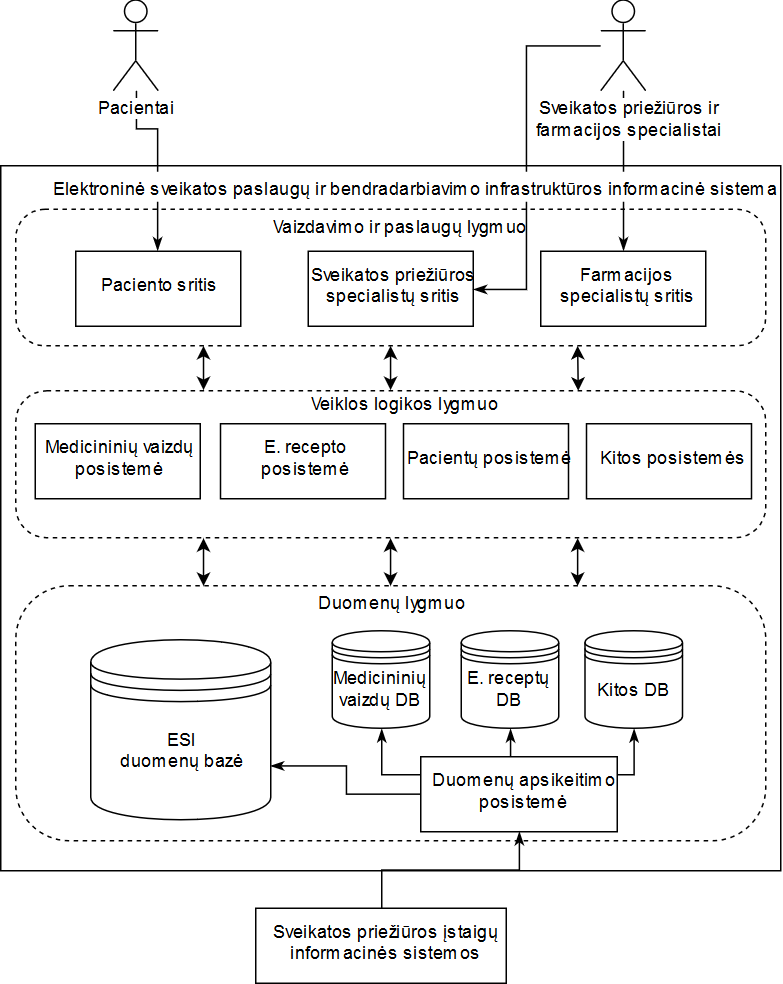
\includegraphics[scale=0.35]{images/ESPBI}
    \caption{Elektroninės sveikatos paslaugų ir bendradarbiavimo infrastruktūros informacinės sistemos achitektūra}   % Antraštė įterpiama po paveikslėlio
    \label{img:ESPBI}
\end{figure}











% issiaiskinti del ruklos, kam ji priklauso ( Jei priklauso kazkam is saraso, galim prideti saltini prie hospitalisation.tex)
% neiasku del duomenu baziu, lape raso, kad ji viena yra, o realiai ju daug